%
%This Skeleton for Master's Thesis reports is written by
%Jonas Birme during his work with his MT-report in 2004.
%Jonas is a former student and Assistant at Computing Science, UmU.
%Jonas is also the author of the documentclass thesis_report.cls
%Both these files have been modified and extended by Per Lindstr�m at Comp. Sc., UmU
%in December 2004.
%
\documentclass[a4paper]{thesis_report}
\usepackage{alltt} 
\usepackage{subfigure} 
\usepackage{longtable}
\usepackage{array,ltxtable,ragged2e}
\usepackage{rotating} 
\usepackage{cancel}
\usepackage[plainpages=false]{hyperref}
\usepackage{url}


\newcolumntype{C}{>{\Centering}X}

\def\lt{{\sc <}}
\def\gt{{\sc >}}

\begin{document}
\pagestyle{empty}

\title{Visualization of Functional Dependencies in a Web Environment}
\author{Nikolay Georgiev}
\credits{15} 
\supervisor{Stephen J. Hegner}
\examiner{Per Lindstr\"om} %Name of examiner (normally Per Lindstr�m}

\pagenumbering{alph}
\maketitle
\cleardoublepage

%%%%%%%%%%%%%%%%%%%%%%%%%%%%%%%%%%%%%%%%
%   Abstract
%%%%%%%%%%%%%%%%%%%%%%%%%%%%%%%%%%%%%%%%
\pagenumbering{roman} \setcounter{page}{1}
\pagestyle{fancy}
\begin{abstract}
Database normalization is a technique for designing relational database tables 
to minimize duplication of information in order to safeguard the database 
against certain types of logical or structural problems, namely data anomalies. 
Therefore database normalization is a central topic in database theory, and its 
correct understanding is crucial for students. Unfortunately  the subject it is 
often considered to be dry and purely theoretical and it is widely being disregarded 
by the students. A web-based learning environment is developed to give 
students an interactive hands-on experience in database normalization process. It
also provides lecturers with an easy way for creating and testing assignments 
on the subject.  
The learning environment is suitable for relational database and design and data 
management courses. 

This report describes the design and development of LDBN 
(Learn DataBase Normalization) - a reference implementation of the learning environment.
It also discuss problems that lie within educational and web-based software development.
A tutorial on the right usage of LDBN is also provided.   
%keywords (do we need them?)
%\newline
%\newline
%\textbf{Keywords:} Database Normalization, Relational Data Model, Functional Dependency, 
%Third Normal Form, Boyce-Codd Normal Form, Embedded Functional Dependencies

\end{abstract}

\cleardoublepage
\begin{spacing}{1.2}
\tableofcontents%
\cleardoublepage

%List of figures and List of tables are not necessary
\listoffigures%
%\listoftables%
\cleardoublepage

\end{spacing}

\pagenumbering{arabic} \setcounter{page}{1}

\chapter{Introduction}
\label{chap:introduction}
Readers unfamiliar with the terms of relational-database normalization and 
functional dependencies can find a brief introduction on the subject in
Chapter~\ref{chap:preliminaries}. 

Due to its great importance for database applications database schema design has
attracted a lot of researchers~\cite{p1}. Relational-database normalization is a 
theoretical approach for organizing data in a database and it is very well developed, 
unfortunately, however, theory does not have much impact on practice yet~\cite{p1}.
One of the reasons for this is the lack of good tools which could aid the students 
during the learning process of relational-database normalization~\cite{p8}. 
Thus our learning environment was developed in order to give students the ability to 
easily and efficiently test
their knowledge of the different normal forms in practice. Moreover, normal forms are formal
notations, which ensure low storage cost and low update cost for databases, they are discussed
more formally in Chapter~\ref{chap:preliminaries}. The environment assists the students by 
providing them the following functionalities:

\begin{enumerate}
	\item Allow the student to specify a candidate decomposition of a given relation.
	\item Assess the correctness of the student's proposed decomposition relative to many factors; including:
		\begin{itemize}
			\item Lossless join property.
			\item Dependency preservation.
			\item Specification of keys.
			\item Correctness of the 2NF, 3NF and BCNF decompositions.
		\end{itemize}
	\item Provide students with sample decompositions when needed. 
	\item Allow users to communicate with each other via comments/posts.
\end{enumerate}

Our learning environment uses many different normalization 
algorithms for achieving the functionalities described above. 
We can divide them into two different groups:

\begin{description}
	\item[Decomposition algorithms] are used for decomposing a normalized database 
	schema into a certain normal form using functional dependencies (FDs).
	\item[Test algorithms] for testing , whether a given relational schema is 
	violating certain normal form, the lossless join property or other criteria.
\end{description}

It is very important to note that the \textit{Decomposition algorithms} are not enough for
our purposes, since they have the 
disadvantage that they could decompose a schema, which is already satisfying 
certain normal form, into a new set of relations/tables~\cite{p4}. Thus there can be many 
possible, distinct decomposition of the same schema, which all satisfy the same 
normal form~\cite{bdb4}. This is a key aspect of the relational-database normalization,
which does not allow us to simply compare the
students' solutions against solutions provided by the decomposition algorithms,
therefore we need the \textit{Test algorithms}.

Here it is worth mentioning that the normalization algorithms often require 
extensive relational algebraic backgrounds that most IS/IT students lack~\cite{p8}. This
is also an issue which our tool is trying to overcome by providing more intuitive 
way of decomposing a schema and by giving an easy way for lecturers to
teach by example and test the knowledge of their students. 

\section{Organization of This Report}
\label{sec:organization}
In the reminig sections of this chapter we are going to informally introduce 
the key features and consepsts of our web-based learning environment, 
called LDBN (Lean DataBase Normalization)~\cite{wldbn}; 
compare it with a couple of other 
available web-based database normalization tools; provide the reader with small glossary.  
The introduction of LDBN in Section~\ref{sec:introldbn} is important for the reader
in order for him/her to better understand the need and the concepts of the algorithms described in 
Chapter~\ref{chap:preliminaries}, where we also give definitions to
relational-database normalization and to the different normal forms. 
In Chapter~\ref{chap:design} we discuss some design issues regarding LDBN like 
platform choice and others. Chapter~\ref{chap:impl} provides a formal description
of our reference implementation of the learning environment. 
Chapter~\ref{chap:conclusion} shows our conclusions, and 
Appendix~\ref{chap:tutorial} contains a simple tutorial to the system.

\section{Learning Database Normalization with LDBN}
\label{sec:introldbn}
In this section we are going to briefly introduce our reference implementation
of the web-based learning environment, called LDBN.    
Figure~\ref{fig:screen01} shows an overview of the most important part of the UI - 
the \textit{Solve Assignment} view/tab. Here students can test their knowledge on 
the subject of relational-database normalization. The first thing the reader 
may notice is the fact that LDBN is running within a browser. The client-side 
of LDBN is written in JavaScript following the AJAX techniques 
(more about this in Chapter~\ref{chap:design}). 
Furthermore, LDBN is assignment driven. This means students have to first 
choose an assignemtn 
form a list with assignments, submitted by other users (lecturers). 
Such a list is shown in Figure~\ref{fig:screen02}. 
Moreover, an assignment consists of a relational-database schema in
universal-relation form (URF), i.e., all the attributes in a single relation 
and a set of FDs on the attributes. 
After an assignment has been loaded, we require the students to go through the 
following steps in LDBN:
\begin{enumerate}
	\item Determine a minimal cover of the given FDs, also known as canonical cover.
	\item Decompose the relational schema from URF into 2NF, 3NF and BCNF. 
	\item Determine a candidate key for each new relation/table. 
\end{enumerate}

\begin{figure}[h]
	\begin{center}
		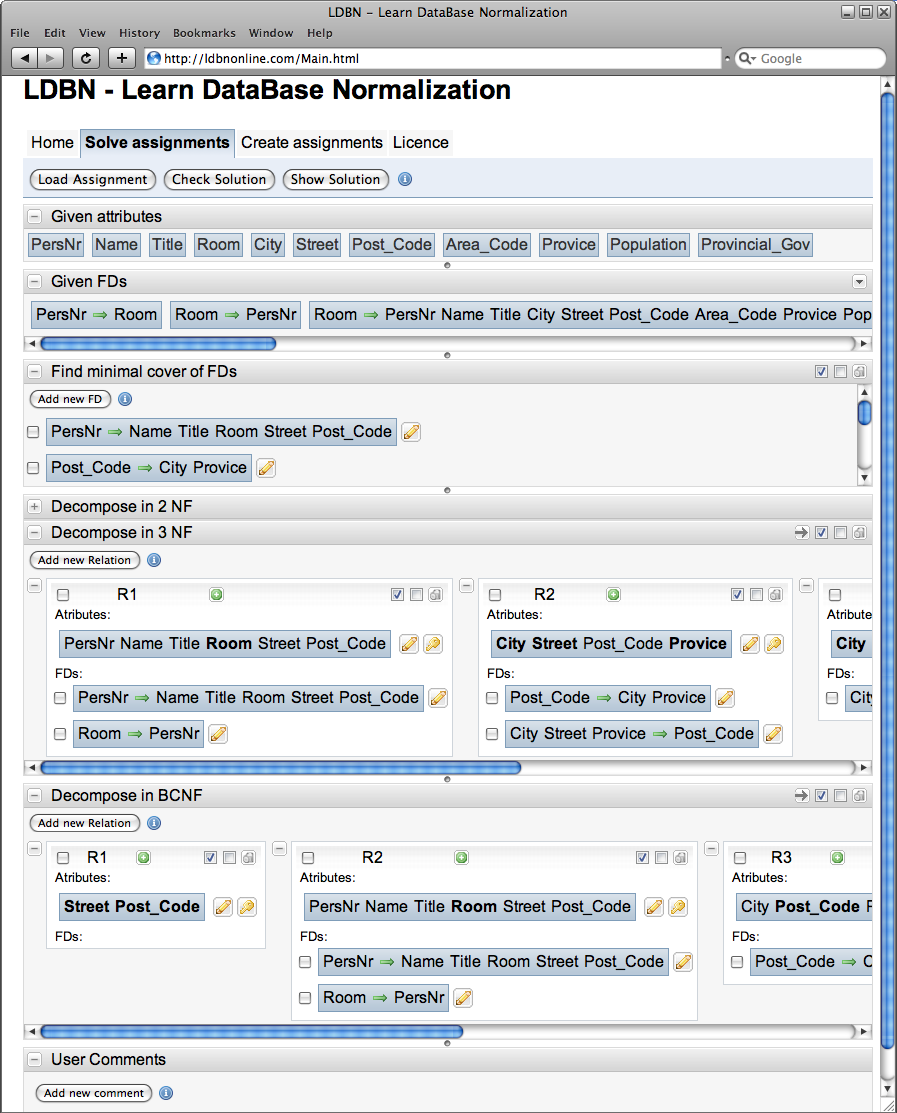
\includegraphics[width=0.8\textwidth]{./img/screen01b.png}
		\caption{LDBN - Solve Assignments Tab}
		\label{fig:screen01}
	\end{center}
\end{figure}

\begin{figure}[h]
	\begin{center}
		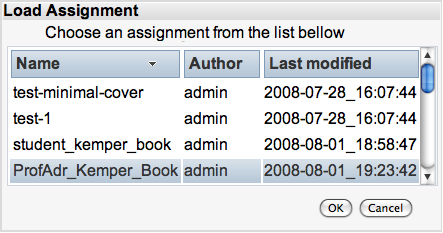
\includegraphics[width=0.6\textwidth]{./img/screen02.png}
		\caption{LDBN - Load Assignments List}
		\label{fig:screen02}
	\end{center}
\end{figure}

The task of checking a potential solution
involves many subtasks which may be performed in any order. In addition to this,  a partial or complete 
solution can be submitted at any given time by pressing the \textit{Check Solution} button. 
After that the system analyzes the solution by performing the following checks:
\begin{enumerate}
	\item Correctness of the minimal cover of the given FDs. 
	\item Losses join properly for every decomposition.
	\item Dependency preservation for every decomposition.
	\item Correctness of the associated with each relation FDs; that is, if the FDs are actually in the embedded closure of F for this relation.
	\item Correctness of the key of each relation.
	\item Correctness of the decomposition, i.e., if the decomposition is really in 2NF, 3NF and BCNF.
\end{enumerate}

\begin{figure}[h]
	\begin{center}
		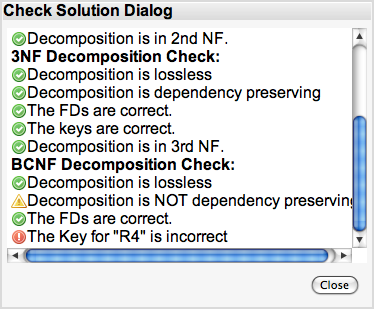
\includegraphics[width=0.6\textwidth]{./img/screen03.png}
		\caption{LDBN - Check Solution Dialog}
		\label{fig:screen03}
	\end{center}
\end{figure}

A dialog with the result is shown to the user. In case of an error the system offers
feedback in form of small textual hints, indicating
where the error might be. Such dialog is shown in Figure~\ref{fig:screen03}. In this case
we can see that the user has made a correct decomposition for 2NF and 3NF,
but his/her decomposition for BCNF has some errors, namely the key of the relation R4 is
incorrect. The dialog is also showing that the decomposition does not 
satisfy the lossless join property, but in the case of BCNF this
is not allays possible, therefore it is only a warning. 

Additional features of LDBN include creating an assignment, which can be done 
only by registered users. This restriction is necessary in order users to be able 
to distinct assignments provided by trusted users, e.g. their database course
lecturers. Registered users have also the ability to leave textual comments 
for every assignment. On the one hand, such
comments ensure that user can easily communicate and share ideas
with each other, and one the other hand, comments could also decrease the amount of workload
for the lecturers in terms of giving an explanation to difficult decomposition.

More detailed and formal description of the features of LDBN will be given in
Chapter~\ref{chap:impl}. 

\section{Comparation of LDBN with Other Tools}
\label{sec:comparation}
In this section we are going to compare LDBN with a couple of other 
available web-based database normalization tools 
such as the \textit{Web-based Tool to Enhance Teaching/Learning Database 
Normalization} by Kung~\cite{p8} and the \textit{The Database Normalization Tool}
\cite{w1}. Furthermore, we are going to discuss why we think our tool is better 
and more efficient
in terms of teaching potential, and give possible reasons why the 
other tools are not commonly used by students.

First of all, the concept of assignments is a major
difference between LDBN and the other normalization tools, 
which only provide 
one possible solution (decomposition) to the user, without users having the ability to test 
themselves. On the other hand, LDBN can be used for checking the correctness of any
arbitrary decomposition, this could be useful for lectures to test handwritten assignments. 

Another major advantage of LDBN over the other tools is the user interface (UI). 
As Frye~\cite{p10} and Dantin~\cite{p9} stated, this is often a
neglected feature, when it comes to educational software. The lack of user-friendly UI 
can often lead to unpopularity of the software among students. An example here could be 
\textit{The Database Normalization Tool}~\cite{w1}. Inputing a relational schema in the program can
take quite sometime due to the fact that
users have to input every attribute manually using the keyboard and then also 
have to input every FD the same way. This may take several minutes even for small  
assignments. Furthermore, relational schemas cannot be saved for future use like 
in LDBN, and users have to input them again next time. To overcome this slow input of user data, 
LDBN supports Drag and Drop. A feature widely used in desktop
applications, but relatively new to AJAX application such as LDBN. Every attribute
and every FD in LDBN can be dragged and dropped, in order 
to define or modify FDs, key attributes, etc... This ensures a really fast and easy
usage of the tool without the need of a keyboard. It should be mentioned
that inputing attributes the traditional way by typing them is also supported.

Community features like posting comments are not present in the other two web-based 
normalization tools, but we believe they are very important when it comes to educational
software. 

\section{Glossary}
\begin{description}
	\item[2NF, 3NF, BCNF] Second Normal Form, Third Normal Form, Boyce-Codd Normal Form. See Section~\ref{sec:nfintro} for more details.
	\item[AJAX] Asynchronous JavaScript And XML is a group of interrelated web development techniques used for creating interactive web applications, for more details see Section~\ref{sec:ajax}.
	\item[CSS] Cascading Style Sheets is a stylesheet language used to describe the presentation of a document written in HTML.
	\item[DBMS] A database management system (DBMS) is a complex set of software programs that controls the organization, storage, management, and retrieval of data in a database.
	\item[GWT] Google Web Toolkit (GWT) is an open source Java software development framework that allows web developers to create AJAX applications in Java. More details in Section~\ref{sec:gwt}.
	\item[ODBC] Open Database Connectivity (ODBC) provides a standard software API method for using database management systems.
	\item[RPC] Remote procedure call (RPC) is an Inter-process communication technology that allows a computer program to cause a subroutine or procedure to execute in another address space.
	\item[SQL] Structured Query Language, is a computer language designed for the retrieval and management of data in relational database management systems, database schema creation and modification, and database object access control management.
	\item[XMLHttpRequest] is an API that can be used by JavaScript and other web browser scripting languages to transfer asynchronously XML and other text data between a web server and a browser.
\end{description}

\chapter{Motivation}
\label{chap:motivation}
The initial version of the learning environment (LDBN 1.0) was used in
conjunction with the course \emph{Principles of Database Systems} at the 
Department of Computing Science at the Ume� University, and some important 
observations were made. In this chapter we present the problems with the 
LDBN 1.0, which were observed during this testing period. 
Some of the problems led to the realization that the learning environment 
needed to be further developed 
%ne mi haresva
and extended in order to allow a more extensive and productive use 
of the system, and in order for the students to be assisted even better 
in the process of understanding the concepts of FDs and 
relational-database normalization by providing new tools to them such as the 
FD visualization tool, which is described in detail in Section~\ref{sec:visualization}.  

\section{Shortcomings of LDBN 1.0}
\label{sec:problem_statement}
At the moment, students, who are trying to solve an assignment with LDBN, often have
to deal with a large number of attributes and FDs based on those attributes. 
However, LDBN 1.0 offers only textual representation of FDs, an example of such
representation is shown in Figure~\ref{fig:exampleFds01} . 

\begin{figure}[ht]
	\begin{center}
		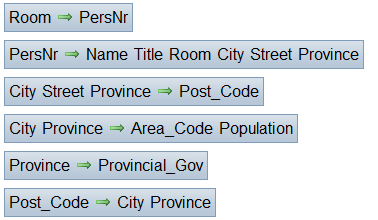
\includegraphics[width=0.7\textwidth]{./img/example_fds_01.png}
		\caption{Example of a Typical Textual Representation of FDs in LDBN 1.0}
		\label{fig:exampleFds01}
	\end{center}
\end{figure}


As can be seen, some attributes 
may occur more than once in a single FD and there may be many different FDs in a single 
assignment. Although this is a standard representation of FDs, 
it may lead to confusion among students and negatively affect the overall
usability of the system. Thus we extended LDBN 1.0 by providing a visualization for
FDs. In order the visualization to be intuitive for 
both students and lecturers we have decided to use templates found in popular 
popular database textbooks such as~\cite{bdb2} and~\cite{bdb1}. 
An example of a such visualization can be observed in Figure~\ref{fig:viz-fds-ex01}, which
was generated with LDBN 1.1. 

\begin{figure}[ht]
	\begin{center}
		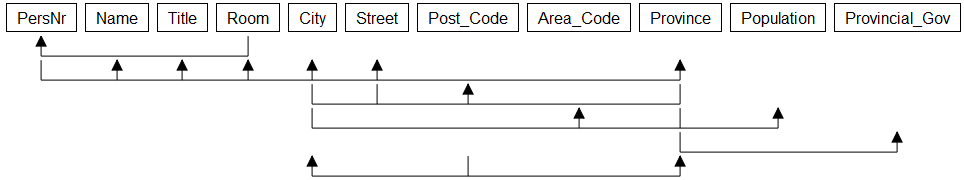
\includegraphics[width=0.95\textwidth]{./img/example_fds_02.png}
		\caption{Example of a Graphical Representation of FDs in LDBN 1.1}
		\label{fig:viz-fds-ex01}
	\end{center}
\end{figure}

Another example of the new visualization functionality can be observed in Figure~\ref{fig:viz-fds-ex02}. 
Figure~\ref{fig:viz-fds-ex02a} shows a set of FDs represented as text in LDBN 1.0, 
and Figure~\ref{fig:viz-fds-ex02b} shows the same set of FDs using the visualization functionality of LDBN 1.1.
The Example is an adaptation of~\cite[Aufgabe~6.7]{bdb2ub}. 
In this case the visualization clearly stands out,
as it delivers a much clearer overview of the FD set. For instance, with the help of the 
visualization one can clearly see that some FDs are redundant, such as $A \rightarrow B$ or $E \rightarrow B C$.
In fact for relatively small sets of FDs, which are typical for LDBN, by using the visualization functionality 
one can easily apply Algorithm~4.12 in~\cite{mt1}, which is used for computing a minimal cover of an FD set -~$F_c$.
In this case a minimal cover may be defined as  
$F_c = A \rightarrow C; E \rightarrow A; F \rightarrow C D; C \rightarrow B E F$. 
Thus all other FDs are redundant, as they may be inferred from $F_c$. 
Readers unfamiliar with the term \emph{Minimal Cover of an FD Set} may refer to~\cite[Section~2.1.6]{mt1}. 

\begin{figure}[ht]
  \centering
  \subfigure[Textual Representation]{
    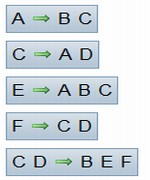
\includegraphics[scale=0.7]{./img/ldbn-viz-ex-fc00.jpg}
    \label{fig:viz-fds-ex02a}
  }
  \subfigure[Graphical Representation]{
    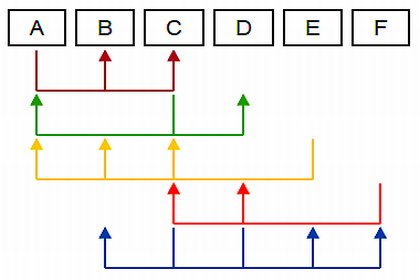
\includegraphics[scale=0.45]{./img/ldbn-viz-ex-fc01.jpg}
    \label{fig:viz-fds-ex02b}
  }
\caption{Example of Different Types of Representation of FDs in LDBN}
\label{fig:viz-fds-ex02}
\end{figure}   

Another major problem with the initial system is the fact that all 
registered users have the same rights. Thus all users can create assignments, which
can be seen by all other registered or unregistered users. In addition, assignments
can be viewed in the \emph{Solve Assignment Tab} only if they have been previously
stored in the system by a registered user. In the original version of the environment (LDBN 1.0),
it was believed that both of these facts would increase the number and the diversity of
assignments stored in the systems, and thus the system would appeal to more students 
and increase usability. 
This collaborative approach has been inspired by the Wikipedia project, where everyone
can be a content contributor and a reader at the same time. 
However, during the testing period the system has been flooded with unsuitable assignments
mainly because of two reasons. First, 
identical assignments occurred more than once under different names. They were usually submitted 
by students in the same class trying to
solve a homework assignment, or just trying the system with examples from textbooks.
Second, users were unable to load an assignment in the \emph{Solve Assignment Tab}
without first storing it in the database of the system, this led to the fact that
users who just wanted to test the system with a simple assignment were in fact
flooding LDBN 1.0 with even more unsuitable assignments, which consist of just a 
few attributes and even fewer FDs, and were of no interest to other users. Both of these
facts led to a major decrease in the usability of the system, 
since students were no longer able to distinguish 
between interesting and well-thought-out assignments submitted by lecturers 
and other assignments. A solution to this problem 
is discussed in detail in Section~\ref{sec:improving}. 
 
\section{Goals}
\label{sec:purpose}
As discussed in the previous section visualization takes a central part in this
thesis. Thus most of the efforts during the implementation period of the project 
were concentrated in delivering a clean and user-friendly visualization of FDs. 
Furthermore, the goals of this thesis can be divided into two parts:

\begin{enumerate}

  \item Implement different types of visualization for FDs based 
  on templates found in popular textbooks such as~\cite{bdb2} and~\cite{bdb1}. 
  Furthermore, the visualization should support different colors schemata and 
  zoom levels for a better presentation. In addition to this, the visualization
  should be available in all fields of the UI which hold a set of FDs. 
  Moreover, it should not interfere with existing representation of the FDs.

  \item Improve the existing system in several ways including:
  
  \begin{enumerate}
    \item Dividing users into at least two groups: 
    (1) instructional users and (2) regular registered users. This is done without
    affecting the existing users, thus all already registered users will keep
    their rights in the system. 
    \item Decrease the number arbitrary assignments by providing new methods for saving and 
    loading assignments in the system. 
    \item Users should be able to delete and edit their previously submitted comments.    
  \end{enumerate}
  
\end{enumerate}

%TODO some more motivation so you can get four pages for this chapter
 
\chapter{Approach}
\label{chap:approach}
In this chapter we discuss some design decisions of our solution such as 
platform choice, as well as a formal overview of our implementation. 

In the following the term client is used to refer to a Web browser.

\section{Choice of Platform}
\label{sec:platform}
This section is, for the most part, a summary of \cite[Section~3.1 and Section~3.2]{mt1}.

There are many different techniques for implementing a Web-based application. 
The problem specifies that the solution must be able on the one hand to 
quickly communicate with LDBN 
and on the other hand to extend some of its capabilities, 
thus a basic HTML solution will not be able to achieve our goal, 
since all pages in that case are static. 

The remaining options can be divided into 3 groups, client-side, server-side and
a client-server based. 

The client-side solutions consist of a Java applet or a Flash
application are downloaded by the browser and then run locally on the computer of the user.
This is achieved by installing a separate browser plug-in. However, this approach has the disadvantage
of requiring a plug-in, which is not always available by default on all Web browsers, and sometimes
installing such plug-ins can only be done by system administrators. This could have a major negative
impact on the usability of the system. 

Server-side includes solutions built in PHP, Perl, ASP, Java, C/C++ or other languages.
This approach
has a centralized architecture, thus all tasks and functions are performed on the server.
After their completion a new static HTML page is sent back to the client.
With this approach the client is unable to remember its state and 
every user interaction causes an HTTP round trip over the network, 
requiring browsers to re-render the whole Web page after each request. With this approach
advanced tasks such as drag and drop, which are heavily used in the initial and current
version of LDBN, become almost impossible to implement due to the high latency time after each
HTTP request. 

The third approach is
a client-server based idea called Asynchronous JavaScript and XML (AJAX),
which is also used by the initial version of LDBN. 
It works almost the same as the server-side solutions but acts more interactively. The
reason for this is the fact that some parts of the program logic are moved from the server
to the client, thus not every user interaction causes necessarily a whole new page
to be rendered. Instead with AJAX the client can request 
data from the server in the background, i.e., without the need to freeze the whole user interface. 
This is usually done by XMLHttpRequest API, which is implemented
by the browser. The API can be accessed by the application using JavaScript, it can be
used to handle communication with the server in an asynchronous fashion over a
simple HTTP connection.
This way after the data is received the client can change only the affected parts of the Web page. 
This on the other hand is once again done by JavaScript, which 
can be used to access and manipulate the DOM of the Web page.
An example of an AJAX architecture is illustrated in Figure~\ref{fig:ajax01}, 
which is an adaptation of~\cite[Figure 3.1]{mt1}.

\begin{figure}[h]
	\begin{center}
		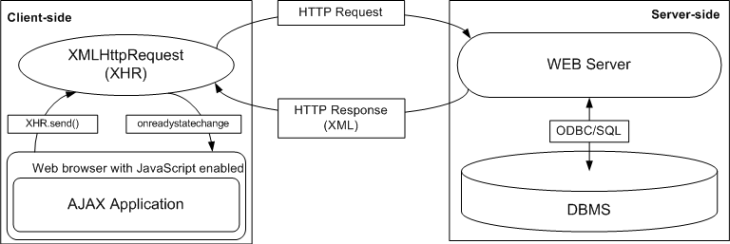
\includegraphics[width=0.8\textwidth]{./img/ajax01a.png}
		\caption{Example of an AJAX Architecture}
		\label{fig:ajax01}
	\end{center}
\end{figure}


It should be noted that AJAX has several shortcomings as well. First of all, 
JavaScript must be enabled in the browser, otherwise the application will not start.
However, the developer can indicate this in the \verb=<noscript>= HTML-tag. 
Nevertheless, the biggest issue with AJAX remains the fact that it is not a
standard. This often requires writing a different code base for different
browsers, and this means less scalability for the application and less productivity for
the developers~\cite{bgwt2}. In the latter case we could avoid some of the issues by using 
Google Web Toolkit (GWT).

\subsection{GWT}
\label{sec:gwt}

GWT is an open source project
and it is developed by Google. It is a set of tools and libraries that allows Web developers to
create AJAX applications in Java. 

The most important component of GWT is the Java-to-JavaScript compiler. It enables the
translation of Java code into highly optimized, browser independent
\footnote{As of GWT version 2.0, GWT supports: 
Firefox 1,~2,~3; Internet Explorer 6,~7,~8; Safari 2,~3,~4; Opera~9,~10, Chrome 1,~2,~3,~4, including mobile browsers for Android and the iPhone.} 
JavaScript code.
In addition to this, it provides developers with compile-time error checking. Another
very important aspect of the compiler is the fact that when the code is compiled into
JavaScript, it results in a single JavaScript file for each browser type and target locale.
This is illustrated in Figure~\ref{fig:gwt01}, which is an adaptation of~\cite[Figure 7]{wgio2}. 
Thus the client downloads and executes only the code that is specifically designed for that platform.  

\begin{figure}[h]
	\begin{center}
		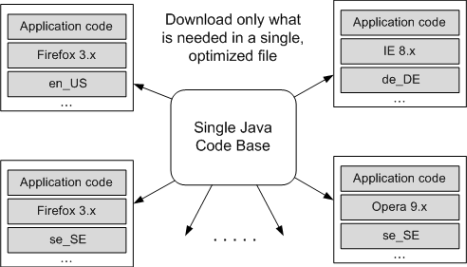
\includegraphics[width=0.8\textwidth]{./img/gwt01a.png}
		\caption{GWT Java-to-JavaScript Compiler}
		\label{fig:gwt01}
	\end{center}
\end{figure}

For additional literature on the subject of GWT, we recommend the book~\cite{bgwt2}. 
It has
proven to be very useful information source throughout the development process 
of LDBN. 

\subsection{Bitmap Rendering with JavaScript}
\label{sec:renderingJS}
When it comes to visualization and graphics in general a more low-level 
pixel control over a certain area of the screen is desired. 
When using JavaScript, however, simple tasks such as drawing a straight
line can become quite challenging in a Web browser environment.
Of course for this purpose we could use client-side solutions, e.g., 
using Flash, or server-side solution, e.g., 
rendering everything on the server as a static image 
and sending it back
to the client. However, for the same reasons as described in the previous
section we decided to use the AJAX approach. This way we can also
adopt a lot of the source code from the previous version of LDBN. 
One way to achieve bitmap rendering with JavaScript is by
using the \verb=<canvas>= HTML-element. 
It is part of the HTML5~\cite{html5} standard, which is the next major revision of HTML, and it is supported by
most of the modern Web browsers. It provides an image-like 
graphics context which can be accessed via a set of JavaScript calls, 
similar to a 2D subset of OpenGL. 
It was originally introduced by Apple in their Safari browser, but it is now 
supported by other modern browser including Mozilla Firefox, Opera and Google Chrome.
It also has better rendering speed than the older Scalable Vector Graphics (SVG) standard~\cite{w8}. 
Unfortunately, Internet Explorer (IE) provides native support for 
neither SVG nor canvas feature of HTML~\cite{w9}. In spite of that, IE does 
implements its own XML-based language for producing vector graphics 
called Vector Markup Language (VML). With the help of VML canvas-specific JavaScript 
calls can be emulated in IE. In LDBN we use the GWT-Incubator project~\cite{gwtincubator}, which provides
browser-independent canvas implementation for GWT projects, thus 
it provides support for all major browsers including IE. 
It should be noted that by doing this
we lose some rendering speed in IE that generally comes in other browsers
with a native canvas implementation. 
On the other hand in our implementation of the visualization of FDs we use only static scenes, i.e., 
no animation or any other intensive 
graphical operations. Therefore, in our opinion, VML is sufficient for our project. 

\section{Implementation}
\label{sec:implementation}
As mentioned earlier the implementation is divided into two parts: 
(1) Visualization of FDs and 
(2) improving the existing capabilities of the system.

\subsection{Visualization of FDs}
\label{sec:visualization}
On the one hand the visualization of FDs is to be the most significant 
part of the thesis. 
On the other hand this extension should not compromise the existing 
user interface of LDBN 1.0. Therefore we decided to
make the visualization available in a separate window in the browser. 
The visualization is then available for every field in LDBN 1.1 which 
holds a set of FDs. In these fields there is an 
icon (
\includegraphics[scale=0.6]{./img/eye.png}) in the upper right
corner, by clicking it we can open the visualization window.
The initial idea
was to implement it as a separate Web application, which can then be 
opened in its own 
browser pop-up window. However, there are two problems with this approach. The first one is
the fact that most of the modern browsers have a pop-up blocker and it is activated by default.
This could have a major negative impact on the usability of the system because there
is always a risk that the user might not notice the pop-up 
warning at all and hence the visualization. The second problem with this approach is 
the fact that we want the visualization to use the existing 
advanced capabilities of LDBN 1.0 such as drag and drop. 
This would have been nearly impossible, though, since
the two application would run in different JavaScript virtual machines for each
browser window. The way around this issue could be the use of a server
which communicates with both applications. However, 
this would make the drag and drop too slow for effective usage. 

In our implementation we use a different approach. We implement our own 
JavaScript-based window package, since GWT does not offer one in its standard library.
With it we can create pop-up windows which exist within a browser window. 
An example of such a window is presented in Figure~\ref{fig:fd-visual-win}. 
Our approach eliminates the previously described problems. First,
the window is part of our JavaScript application and as such it does not 
trigger any bowser pop-up blockers. 
Second, the visualization and the LDBN system can directly share any 
JavaScript objects, since they run in the same virtual machine, 
this way they can interact in a very fast and efficient way. 
This is very similar to the pop-up dialogs used in the initial version of our learning environment (LDBN 1.0). 
These dialogs are provided in the standard widget library of GWT. 
However, they prove to be inconvenient for our needs, since once created and attached 
to the DOM they cannot be resized. On the other hand, we
need this kind of resize-window functionality since we want to offer the user
different zoom levels for the visualization, as well as the ability the user to resize the
visualization window, since they could become quite large and hide important parts of the user 
interface. Furthermore, with our implementation we have more powerful control over
the graphical representation of the window. This way for example we can add a close button (image)
in the upper right corner, which is a more intuitive way to interact with the UI.

\begin{figure}[h]
	\begin{center}
		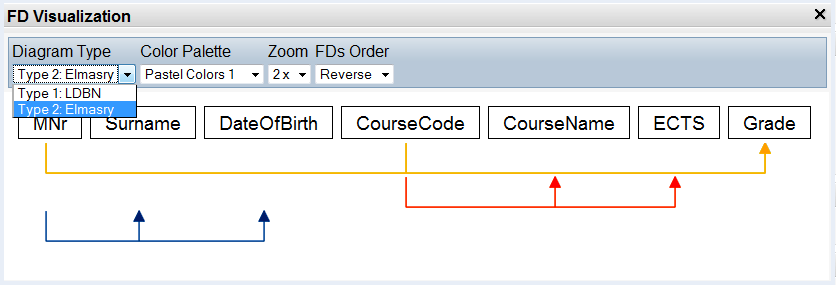
\includegraphics[width=0.9\textwidth]{./img/fd-visual-win.png}
		\caption{FD Visualization Window}
		\label{fig:fd-visual-win}
	\end{center}
\end{figure}

At the implementation level the visualization consists of two components. 
Both of them are illustrated in Figure~\ref{fig:impl-fds01}.
The first component is a simple GWT panel where all the attributes of an FD are displayed. 
Internally the attributes are represented as GWT widgets, thus the rendering of those attributes is
handled by the browser. In fact, these are the same widget classes used for representing
attributes in the \emph{Given Attributes} field, which is shown in Figure~\ref{fig:given-atts}. 
The only difference between the two kinds of attribute representations is 
that we apply a different CSS style sheet for each of them. By using the already implemented in LDBN 1.0 
widget classes we get advanced functionality such as drag and drop for free. Thus the user
can drag any attribute in the visualization window and drop 
it in the text box of the different editors in LDBN
such as the \emph{Attribute Editor} or the \emph{FD Editor}, the latter is 
shown in Figure~\ref{fig:fdeditor}. 
As a result the
attributes are automatically inserted in the text areas of the editor and users do not have
to type them by hand, which for long attribute names could become inconvenient and error prone. 
We believe the drag and drop functionality can help
users define attributes, keys or FDs much more quickly, which can
help improve the usability of the learning environment.

\begin{figure}[h]
	\begin{center}
		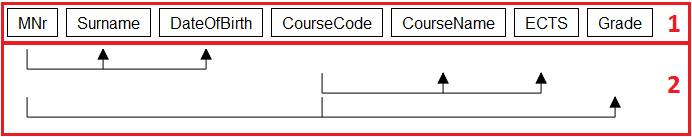
\includegraphics[width=0.9\textwidth]{./img/impl-fds01.png}
		\caption{Visualization Components}
		\label{fig:impl-fds01}
	\end{center}
\end{figure}

\begin{figure}[h]
	\begin{center}
		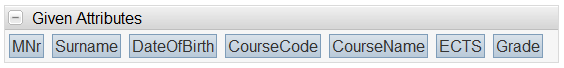
\includegraphics[width=0.9\textwidth]{./img/given-atts.png}
		\caption{Given Attributes Widget}
		\label{fig:given-atts}
	\end{center}
\end{figure}

\begin{figure}[h]
	\begin{center}
		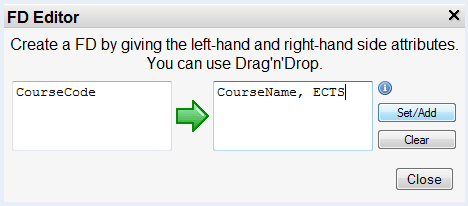
\includegraphics[width=0.6\textwidth]{./img/fdeditor.png}
		\caption{FD Editor Dialog in LDBN}
		\label{fig:fdeditor}
	\end{center}
\end{figure}

The second component of the visualization consists of a \verb=<canvas>= HTML5-element. 
It is shown in Figure~\ref{fig:impl-fds01}.
The canvas element is placed bellow the attributes, and there the actual drawing 
of the FDs takes place. In LDBN we support two types of visualization, each of them can be selected
from the \emph{Diagram Type} drop down menu in the visualization window. The first type is called 
\emph{Elmasti}, since it is the form of representation used in~\cite{bdb1}. 
The main difference between this approach and
the traditional representation of FDs is the fact the we display each attribute in the set of 
FDs only once. 
Similar to the purely text-based representation we can visualize the set
of FDs as a set of rows. Each row representing one FD of the set. 
However, in this visualization all attributes that occur in the set of FDs
are shown in the first row. Then every FD is displayed in a separate row by an outgoing 
arrow for each attribute from the left-hand side (LHS) of the FD,
and as an incoming arrow for the attributes of the right-hand side (RHS).

This approach is quite intuitive and we believe it will be well received by
students, since during their database courses at the university most of 
them get familiar with~\cite{bdb1}, from which
the visualization is inspired. However, the approach has some disadvantages
as well, not the least of which is the fact that it does not make use
of all the available white space in the diagram. To address this issue
we offer a option where the user can change the order in which
the FDs are rendered. In addition to this, we also offer another type of
visualization where the arrows of each FD always start/reach the 
attributes at the top of the diagram. 
Both types of visualization can be observed in 
Figure~\ref{fig:dia_example_elmasry} and~\ref{fig:dia_example_ldbn}.

\begin{figure}[h]
  \centering
  \subfigure[Type: Elmasri]{
    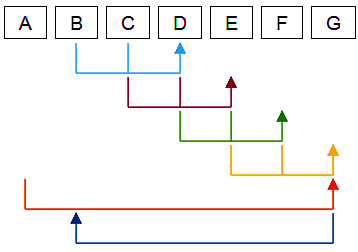
\includegraphics[scale=0.5]{./img/dia-elmasri-ex-fds-01.png}
    \label{fig:dia_example_elmasry}
  }
  \subfigure[Type: LDBN]{
    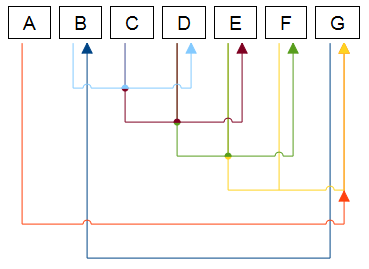
\includegraphics[scale=0.47]{./img/dia-ldbn-ex-fds-01.png}
    \label{fig:dia_example_ldbn}
  }
\caption{Diagram Types in LDBN}
\end{figure}

Certainly another important aspect in visualization in general are colors.
In our visualization we offer five different color palettes. The user can 
choose between:
\begin{enumerate}
	\item \emph{Black Only} - All FDs appear black. This is useful for printing
	purposes.
	\item \emph{Gray Shades} - Each FD appear in a different color tone of gray. 
	At this point is should be noted that when compared with other colors 
	the human eye can detect best shades of gray, and on a modern LCD screen it can
	distinguish between 30 shades of gray~\cite[Chapter 2]{bimg1} . 
	\item \emph{Pastel Colors} - Here we use less saturated colors which appear pastel. 
	Colors codes are taken from~\cite{wpastel}.
	\item \emph{Standard Colors} - The standard color palette consists of predefined
	HTML colors such as reg, green, blue, etc. These colors often appear vivid 
	(highly saturated colors).
	\item \emph{OpenOffice Style} - In this  palette we use colors which
	can be found in charts created with the help of OpenOffice.org~\cite{wooorg}. 
\end{enumerate}
 
% Color Contrast 
% see http://snook.ca/technical/colour_contrast/colour.html
% http://www.w3.org/WAI/WCAG20/quickref/#qr-visual-audio-contrast-contrast
% http://www.w3.org/TR/2008/NOTE-WCAG20-TECHS-20081211/G18

Another important issue when using colors is contrast. 
According to the W3C guidelines a Web application should use such
foreground and a background colors that provide enough of a
contrast \emph{``when viewed by someone having color deficits or when 
viewed on a black and white screen``}~\cite{w3c1}.
To ensure these property we use WCAG 2.0 contrast ratio formula~\cite{w3c2}.
Our color palettes are WCAG 2 AA Compliant for text larger than 18pt.

As can be seen in Figure~\ref{fig:fd-visual-win}, 
the visualization feature offers a magnification function as well. 
Thus the user can zoom in and out on a diagram.
This is practical especially when a
diagram contains a lot of attributes and the user 
wants to get a general idea of the FDs, then 
he\footnote{``He`` should be read as ``he or she`` throughout this thesis.} can
simply zoom out. 
The zoom functionality
is achieved by applying different CSS with different font 
size for the attributes and by redrawing the canvas element accordingly. 

\subsection{Improving the Usability of LDBN}
\label{sec:improving}

Another major part of this thesis is the improvement of the
existing functionality of the learning environment. 
To address some of the issues described in 
Section~\ref{sec:problem_statement} we introduced a more sophisticated user system in 
LDBN 1.1. In the previous version of the system all user had the same rights. 
In the current version we introduce following three groups of user:
(1) \emph{Regular Users}, (2) \emph{Instructional Users}, and (3) \emph{Superusers}.

Furthermore, each user group has different rights in the system. 
Table \ref{tab:user-rights} shows the different user rights in LDBN 1.1 for each user group. 

\begin{center}
\begin{table}
\begin{tabular}[h]{| m{2.8cm} || m{2.2cm} | m{3.2cm} | m{3.3cm} |}
\hline
 & \textbf{Regular Users} & \textbf{Instructional Users} & \textbf{Superusers} \\
\hline
\hline
\emph{Create \mbox{Assignments}} & Yes & Yes & Yes \\
\hline
\emph{Edit \mbox{Assignments}}  & Only their own & Their own and assignments submitted by regular users & Their own and assignments submitted by regular or instructional users \\
\hline
\emph{Delete \mbox{Assignments}} & No & Their own and assignments submitted by regular users & Their own and assignments submitted by regular regular or instructional users \\
\hline
\emph{Leave \mbox{Comments}}    & Yes & Yes & Yes \\
\hline
\emph{Edit \mbox{Comments}}     & Only their own & Their own and comments submitted by regular users & Their own and comments submitted by regular or instructional users\\
\hline
\emph{Delete \mbox{Comments}}   & Only their own & Their own and comments submitted by regular users & Their own and comments submitted by regular or instructional users \\
\hline
\emph{Add Users to the Group of \mbox{Instructional Users}} & No & Yes & Yes \\
\hline
\emph{Remove Users from the Group of \mbox{Instructional Users}} & No & No & Yes \\
\hline
\end{tabular}
\caption{User Rights in LDBN 1.1}
\label{tab:user-rights}
\end{table}
\end{center}


Under the hood LDBN manages the user data in a MySQL database. 
We realize the different user groups by simply altering the already existing table \verb=users=. 
and adding two more attributes 
of type boolean - \verb=isInstructionalUser= and \verb=isSuperuser=. 
These attributes are set to \verb=true= when a user has instructional users and respectively superuser 
rights in the system. 

Furthermore, in order to make it easier for instructional and superuser to manage the system
we develop an extra user interface (UI) in LDBN called \emph{Administrators}, which is accessible via a
separate tab. It can be seen in Figure~\ref{fig:admin-ui}. 
The \emph{Administrators} UI offers three buttons which open 
different dialogs for adding/removing users to/from the instructional user group and for
deleting assignments. Creating and editing assignments can still be done in the 
\emph{Create Assignments} tab. Furthermore, superusers rights can only be realized by making
a corresponding SQL statement for a specific user. However, this is not an issue, since 
we do not expect the system to have more than one or two superusers. 

\begin{figure}[h]
	\begin{center}
		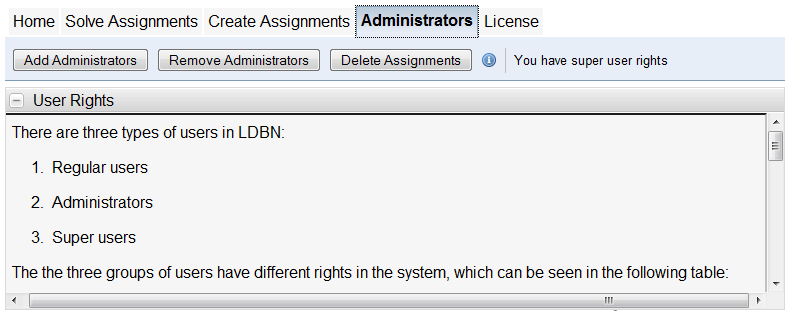
\includegraphics[width=0.9\textwidth]{./img/admin-ui.png}
		\caption{Administrators Tab}
		\label{fig:admin-ui}
	\end{center}
\end{figure}

With the new separation of users into groups we can easily overcome most of 
the issues surrounding user privileges described in the Section~\ref{sec:problem_statement}.
Most importantly, we implement different filters for the \emph{Load Assignment} dialog,
which can be seen in Figure~\ref{fig:load-assg}. The user can choose from 
a drop-down menu to show only assignments submitted by instructional users 
(or superusers), the user himself or to show all assignments stored in the system. 
In addition, it should be noted that only assignments submitted
by instructional and superusers are visible by default, since instructional are in most
cases course lecturers and they provide more sophisticated and 
well-thought-out assignments. 

In order to view other assignments, which are present in the system, 
one should choose a different filter from the drop-down menu. 
On the one hand, we implement the filters on the client-side, thus when a new filter is
applied we do not cause a new server interaction. Rather we apply them
on the initially received dataset, which holds all the meta data for each assignment.
On the other hand, this makes the UI very responsive to user input. 
In order to further increase the usability of the \emph{Load Assignment} dialog
we implement a column-soring function for it. As a result, users can click on
the different headers such as \emph{Name, Author and Last Modified} and sort the 
assignments correspondingly in an increasing or in a decreasing order. This is once
again done on the client side. 

\begin{figure}[h]
	\begin{center}
		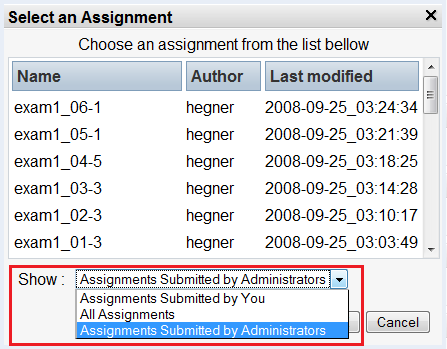
\includegraphics[width=0.6\textwidth]{./img/load-assg.png}
		\caption{Load Assignment Dialog with Filters}
		\label{fig:load-assg}
	\end{center}
\end{figure}

To decrease the number of assignments submitted to the system we added a new button
in the \emph{Create Assignments} tab called \emph{Load in SA Tab}, 
which can be observed in Figure~\ref{fig:load-in-sa}. 
In this case \emph{SA Tab} means \emph{``Solve Assignments Tab"},
which is the tab/view in the system, where students can test their knowledge by solving assignments. 
With the addition of this feature it is now possible to create an assignment and load it 
in the \emph{Solve Assignments} tab without
the need to first store it in the database. Moreover, users do not have to register or 
to log-in in order to use this
functionality. This new feature in LDBN 1.1 is especially useful for users who 
just want to get a general overview of the system and
do not want to become contributors, 
or for testing purposes for users who are currently creating an assignment. 

Another useful feature in LDBN 1.0 is support for user comments, 
which users can give for each assignment. These comments
are then shown in the \emph{Solve Assignments} tab when the assignment is loaded. On the one
hand, such comments ensure that users can easily communicate and share ideas with each
other, and comments could also decrease the amount of workload
for the lecturers in terms of giving an explanation to a difficult decomposition. However, in LDBN 1.0  
once submitted comments could not be altered. The only way to edit or to delete a
comment was to make the corresponding change directly in the database of the system. 
In the new version of our implementation (LDBN 1.1) 
users can edit and delete comments directly via the UI. When a user has
the rights to make a change on a comment or to delete it a corresponding icon is shown 
(
\includegraphics[scale=0.7]{./img/edit.png} or 
\includegraphics[scale=0.7]{./img/del.png})
next to the comment entry.

\begin{figure}[h]
	\begin{center}
		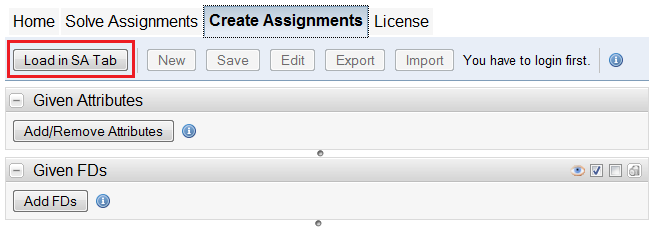
\includegraphics[width=0.75\textwidth]{./img/load-in-sa.png}
		\caption{Load in SA Tab Button}
		\label{fig:load-in-sa}
	\end{center}
\end{figure}

\chapter{Conclusions}
\label{chap:conclusion}


\chapter{Acknowledgements}
\label{chap:acknowledgements}
I would like to thank my supervisor, Stephen J. Hegner, who has supported me 
throughout my thesis with his patience and knowledge 
while allowing me the room to work in my own way. 
Without him this report would not have been completed.

I would also like to thank Michael H\"ofling for all his help during my stay in Sweden.
Last, and most importantly, I thank my family for their love and support.

%
%In order to use the bibliography{base}-command you have to prepare a "database"
%base.bib in a certain format and then run the bibtex-command (a Unix-command) to create
%a file base.bbl which LaTeX uses to create References
%
\cleardoublepage
\addcontentsline{toc}{chapter}{References}
\renewcommand{\bibname}{References}
\bibliographystyle{plain}
\bibliography{./tex/base}

%\appendix
%\chapter{Tutorial}
\label{chap:tutorial}
A tutorial to the right usage of LDBN. 
 

\end{document}
